% Simo.Nikula@gmail.com
% based on latex template at http://www.lut.fi/web/en/library/dissertations1 
\def\mytitle{Handling of plasticity in physics engine}
\def\myisbn{978-952-265-XXX-X}
\def\mypdfisbn{978-952-265-XXX-X}
\def\myyear{2017}
\def\mymonth{May}
\def\myname{Simo Nikula}
\def\lut{Lappeenranta University of Technology}
\def\bullet{Bullet Physics}
\def\demolisher{DemolisherDemo}
\def\charpy{CharpyDemo}
\documentclass[a4paper,twoside,12pt,notitlepage]{article}
\usepackage[utf8]{inputenc}
\usepackage{graphicx}
\usepackage{natbib}
\usepackage{lastpage}   % page count
\usepackage{amsmath}
% \usepackage{mathdots}  % improved \ddots and \iidots
\usepackage{amssymb}
\usepackage[english]{babel}
\usepackage[intoc]{nomencl} % including table of content
\usepackage{ifthen}
\usepackage[hmargin=2.0cm,vmargin=1.6cm]{geometry} % setting marginals
\usepackage{fancyhdr,extramarks}  % header ja footer manipulation
\usepackage{times}  % to change font to times
\usepackage{setspace} % for linespacingx
\usepackage{tikz}
\usetikzlibrary{arrows}
\usetikzlibrary{arrows.meta}
\usepackage{caption}
\usepackage{varwidth}
\usepackage{enumitem} % 
\newcommand{\nomunit}[1]{\renewcommand{\nomentryend}{\hspace*{\fill}#1}} % Inserts units on the right at symbol list
\renewcommand{\nomgroup}[1]{%
 \ifthenelse{\equal{#1}{C}}{\item[\textbf{Latin alphabet}]\item}{%
 \ifthenelse{\equal{#1}{G}}{\item\item[\textbf{Greek alphabet}]\item}{}}{%
 \ifthenelse{\equal{#1}{L}}{\item\item[\textbf{Subscripts}]\item}{}}{%
 \ifthenelse{\equal{#1}{H}}{\item\item[\textbf{Superscripts}]\item}{}}{%
 \ifthenelse{\equal{#1}{W}}{\item\item[\textbf{Abbreviations}]\item}{}}{}}

\singlespacing

\pagestyle{fancy}
\fancyhf{}% clearing the header and footer
\fancyhead[LE,RO]{\bfseries\thepage}    % page number to header
\fancyhead[LO]{\nouppercase{\bfseries\rightmark}}     %
\fancyhead[RE]{\nouppercase{\bfseries\leftmark}}%

\renewcommand\sectionmark[1]
 {\markboth{\thesection\ #1}{}}         % section name to header
\renewcommand\subsectionmark[1]
 {\markright{\thesubsection\ #1}}       % subsection name to header
\renewcommand{\headrulewidth}{0.5pt}    % ruler thickness between head and body
\renewcommand{\footrulewidth}{0pt}      % no ruler between body and footer

\setlength{\nomitemsep}{-\parsep}   % removing default extra skip between entries at nomenclature

\numberwithin{equation}{section}    % equation numbers with section numbers
\numberwithin{table}{section}       % table numbers with section numbers
\numberwithin{figure}{section}      % figure numbers with section numbers

% makeindex command needs to run at command prompt to create nomenclature list file
\makenomenclature % makeindex main_v2.nlo -s nomencl.ist -o main_v2.nls
%\bibpunct{(}{)}{;}{a}{,}{,}%

\begin{document}

\pagestyle{empty}
\title{\mytitle}
\author{Simo Nikula, Aki Mikkola and Timo Björk}
\author{}
\maketitle
% !TeX root = article.tex
\begin{abstract}
We introduce simple and efficient method to simulate ductile fracture in existing physics engines.
Method is based on common technique of splitting bodies to multiple pieces.
\end{abstract}

\section{Introduction}

Computational techniques used in modern computer games are able to describe
complex dynamic systems such as those found in military and other motorized vehicles
with a high level of accuracy while still being able to solve the equations of motion in real time.
Film production and the computer game genre of war games
are two areas that have greatly benefited from rapidly improving simulation technology. 
In practice, software for such games is often written using open-source physics engine platforms  
like ODE - \cite{ode}, \cbullet\ - \cite{bullet} and Box2D - \cite{box2d}.

Computational methods used in physics engines are divided into modules that handle collision detection and 
contact description and modules that handle solution of equations of motion in real time. 
The equations of motion that need to be 
solved can be subdivided into equations related to motion, constraints and collisions. 
Velocity-based formulation is typically used in constraint based rigid body simulation, \cite{erleben.thesis}. 
Friction is typically taken into account and mechanical joints are handled by constraint equations,
\cite{erleben.thesis}.

Plasticity is not typically taken into account in gaming solutions and 
destruction of various bodies often takes place based on collision or impulse exceeding predefined limit.
Nevertheless, breaking of steel or reinforced concrete structures using this approach 
is not appropriate if the simulation is to look realistic. Theory for handling of plasticity 
has been presented already in \cite{cg1988}. 
\cite{Jones:2016:EPD} provides extensive listing of related work during past decades.
\cite{muller2005meshless} 
present a method for modeling and animating of elastic and plastic bodies in real time using 
point based animation. This approach has not been widely used in computer games.  
One major issue is collision handling of deformable bodies.
Recently there has been multiple studies which have same target of bringing plasticity 
into main stream games as this work, \cite{Jones:2016:EPD,Patkar:2015:EDB,Budsberg:2014:EPD}.

This study will introduce an approach to account for plastic deformation in game applications.   
In the introduced method, plastic deformation takes place if the force or moment exceeds a predefined 
limit, deformation absorbs energy and joint breaks if plastic capacity is exceeded. 
The approach is based on using joint motors to model plasticity. 
The study extends a method introduced by
\cite{erleben.thesis} 
%\citet[p.~90]{erleben.thesis} 
which was originally proposed for modelling friction in joints. 
In the introduced method adjacent bodies are connected by motors. 
Motor power production limits are estimated based on the plastic section modulus. 
Joint breaking is based on summing plastic deformation and comparing it to a
predefined material based limit. The elastic part of deformation is modelled by employing 
a spring based on modification of an existing constraint in \cbullet.

The approach presented in this work can be used in the gaming industry to provide more realistic 
simulations without significant extra work. For gaming purposes, the presented method works 
best in scenarios where the connected parts are heavy. This allows a normal 
integration timestep to be used without stability issues. 
This methodological approach enbles established structural analysis
methods to be combined with modern simulation frameworks.


\section{Using physics engine for structural analysis}

Velocity-based formulation is not typically used in structural or mechanical engineering.
 \citet[p.~45]{erleben.thesis} provides reasoning and theoretical details why it is so popular in 
constraint-based rigid body simulation. 
Main reason is that collision handling can be done without additional procedures.
In structural finite element analysis solution method is selected carefully based on needed features.
In most cases static small displacement solution using displacement based boudary conditions is used.
For large displacement static analysis analysis loading is applied in substeps and 
displacements are used to update element mesh.
Further enhancements are material nonlinearity and dynamic analysis.
Physics engine provides dynamic analysis with large displacements.

Material plasticity has typically taken into account in games by using suitable coefficient of restitution.
This provides reasonable means to simulate loss of energy in collisions.
Simulation of breaking of objects made of ductile material can be made more realistic by splitting rigid objects
to multiple parts which are connected by energy absorbing joints.
As stress-strain curve may not be familiar to all readers some basics are provided here.
Typical stress strain curve of ductile steel is shown in \ref{fig:areas}.
Stress-strain curve is not drawn to scale as elastic strain could not be seen as it is typically 0.001 to 0.005.
Straing hardening is taken into account mainly by assuming that plasticity in bending expands.
Material that starts to yield first is hardened and yielding moves slightly.
This can be seen e.g. by bending paperclip. It does not break at low angles but can take few full bends. 

\begin{figure}[htb!]
\centering
\begin{tikzpicture}
\coordinate (Y) at (0.2,4);
\draw[->] (0,0) -- (10,0) node[right] {\large{$\epsilon$}};
\draw[->] (0,0) -- (0,6) node[above] {\large{$\sigma$}};
\draw(0,0) -- (Y) -- (2,4) .. controls (7,6) .. (10,5);
\draw[dashed](0,4) -- (Y);
\node at (-0.2,4) [align=right] {$f_y$};
\end{tikzpicture}
\caption{Stress-strain curve of ductile steel (not to scale).}
\label{fig:areas}
\end{figure}

Difference between elastic and plastic section modulus is shown in \ref{fig:wp}. 
If stress is below yield limit, stress and strain are linear within cross section.
If cross section is fully plastic, stress is assumed to be at yield level over whole cross section and 
so plastic section modulus is higher than elastic section modulus.
Elastic part is often ignored in this work as displacements due to to elastic deformation are very small.

\begin{figure}[htb!]
\centering
\begin{tikzpicture}
\coordinate (S) at (2.5,5);
\draw (0,5) -- (4,5) ;
\draw (0,0) -- (4,0) ;
\draw (2,0) -- (2,5) ;
\draw (1.5,0) -- (S); 
\node[above] at (S) [align=center] {\large{$\sigma<f_y$}};
\end{tikzpicture}
\hspace{1cm}
\begin{tikzpicture}
\coordinate (S) at (3,5);
\draw (0,5) -- (4,5) ;
\draw (0,0) -- (4,0) ;
\draw (2,0) -- (2,5) ;
\draw (1,0) -- (1,2.5) -- (3,2.5) -- (S); 
\node[above] at (S) [align=center] {\large{$\sigma=f_y$}};
\end{tikzpicture}
\caption{Stress distribution under elastic and plastic loads.}
\label{fig:wp}
\end{figure}

Basic idea in this work can be tested with any framework having motors and hinge constraints.
This can be done by setting target velocity of motor to zero and limiting maximum motor impulse to plastic moment 
multiplied by timestep.

Further enhancements were created and tested by forking \bullet\ source code
and adding new constraints \cite{pbullet}.
Constraint processing in \bullet\ is based on ODE, \cite{ode}.
Mathematical background and detailed examples are available by \cite{ode.joints}.
Equations \ref{eq:constraintEquation}, \ref{eq:lambdaLow} and
\ref{eq:lambdaHigh} 
are created for each constraint.

\begin{equation} \label{eq:constraintEquation}
J_1 v_1 + \Omega_1 \omega_1 + J_2 v_2 + \Omega_2 \omega_2 = c + C \lambda
\end{equation}

\begin{equation} \label{eq:lambdaLow}
\lambda \geq l
\end{equation}

\begin{equation} \label{eq:lambdaHigh}
\lambda \leq h
\end{equation}

Main parameters  and corresponding fields in \bullet\  
 are described in table \ref{tab:constraintParameters}.

\begin {table}[htb!]
\begin{center}
\begin{tabular}{|c| l| l|}
\hline
{\bf Parameter} & {\bf Description} & {\bf btConstraintInfo2 pointer}\\  \hline
$J_1, \Omega_1$ & Jacobian & m\_J1linearAxis, m\_J1angularAxis \\ 
$J_2, \Omega_2$ & & m\_J2linearAxis, m\_J2angularAxis \\ \hline
$v$ & linear velocity & \\ \hline
$\omega$ & angular velocity & \\ \hline
$c$        &  right side vector   & m\_constraintError \\ \hline
$C$  & constraint force mixing & cfm \\  \hline
$\lambda$ & constraint force &  \\ \hline
$l$ & low limit for constraint force & m\_lowerLimit \\ \hline
$h$ & high limit for constraint force & m\_upperLimit \\ \hline
\end {tabular}
\end{center}
\caption {Constraint parameters} \label{tab:constraintParameters} 
\end {table}
% !TeX root = article.tex
\section{Numerical examples}

\subsection{Block under tension}
In this section, changes to the constraint formulation are exemplified with some simulation steps
of non constrained, rigid and
elastic-plastic examples using numerical values.

\begin{figure}
\centering
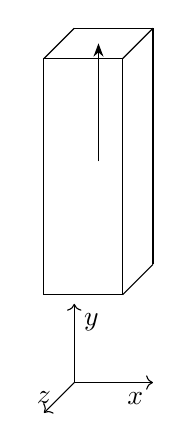
\begin{tikzpicture}
\coordinate (O) at (0,0,0);

% axes
\draw[->] (O) -- (1,0,0) node[anchor=north east]{$x$};
\draw[->] (O) -- (0,1,0) node[anchor=north west]{$y$};
\draw[->] (O) -- (0,0,1) node[anchor=south]{$z$};

% 1,3,1 block, base at y=1.5
\draw (1,1.5,0) -- ++(0,3,0) -- ++(-1,0,0);
\draw (0,1.5,1) -- ++(1,0,0) -- ++(0,3,0) -- ++(-1,0,0) -- ++(0,-3,0);
\draw (1,1.5,0) -- ++(0,0,1);
\draw (0,4.5,0) -- ++(0,0,1);
\draw (1,4.5,0) -- ++(0,0,1);

\draw[-Stealth] (0.5,3,0.5) -- ++(0,1.5,0);
\end{tikzpicture}
\caption{Single body model for plasticity processing.}
\label{fig:tensionModel}
\end{figure}

In the first example, the system under investigation
has only one dynamic rigid body which is a three meters high block of 0.04 \% steel enforced concrete. 
The cross section is one square meter.
A constraint is set so that the connecting frame is at the top of the block. 
In this case, the frame could be anywhere but if multiple bodies are involved, the connecting frame must be defined
so that it reflects the scenario under investigation.
Concrete density is $2000\ \frac{kg}{m^3}$ and steel density is $7800\ \frac{kg}{m^3}$. 
Steel is assumed to handle load in the elastic-plastic case. The yield stress of steel is 200 MPa.
Gravity is $10\ \frac{m}{s^2}$ to keep numbers simple. 
Simulation step is $\frac{1}{60}\ s$ and 10 
iterations are done for a single step.
The body is 1.5 meters above rigid ground. In the unconstrained case the body will hit hit the ground at $t$ = 0.548 s 
($\sqrt{2 \cdot 1.5 / 10}$).

A single simulation step is performed using the following substeps. 
In this work, changes are made only to the constraint setup and the update actions.
\begin{enumerate}
\item Apply gravity to each moveable body. 
This step makes programming easier as otherwise each program should add forces due to gravity in each step. 
In this case, $\vec{f}_{ext}$ in  Equation \ref{eq:eomV2} is added by $\lbrace{0,-60000,0}\rbrace$.
\item Predict unconstrained motion for each body controlled by the physics simulation.
Static and kinematic bodies are not processed in this step.
Prediction is done based on current linear and angular velocities of the body.
\item Predict contacts. In this phase, continuous collision detection is done based on simplified bodies. 
Each rigid body is represented by sphere geometry and contact prediction is done if 
the body moves more than a given threshold value during the simulation step. 
Continuous collision detection is configured for each body. 
A typical scenario that requires continuous collision detection is fast moving bodies that would otherwise go through walls.
\item Perform discrete collision detection. All overlapping bodies are processed and manifoldPoints are created for
each detected contact at the end of the simulation step. 
In the unconstrained case, contact is detected after $t$=0.55 s if 
continuous collision detection is not used and manifold distance gets a negative value (-0.058 m).
\item Calculate simulation islands(groups). Bodies that are near each other based 
on contact prediction or discrete collision detection
 or connected with constraints are grouped in the same group.
\item Solve constraints. Both contact and other constraints are processed in this step. 
 This step is subdivided to setup, iterations and finish phases. 
In teh setup phase constraints are queried for positional errors for calculation of $c$ in
Equation \ref{eq:constraintEquation} and maximum and minimum impulses in Equations \ref{eq:lambdaLow} and 
\ref{eq:lambdaHigh}.
In the finish phase constraint forces are calculated if requested and velocities of bodies are updated.
\item Integrate transforms using velocities modified in the previous step.
\item Update actions (callbacks) are called. 
In the elastic-plastic case, plasticity is summed and the equilibrium
point of the elastic part is updated if the maximum force or moment is exceeded.
\item Activation state of bodies is updated. 
To avoid extra calculation bodies are as default put into sleeping state if linear and angular velocities of
the body are less than
given threshold values (default 0.8 and 1.0) or longer than the set time limit (2.0).
\end{enumerate} 

Equation \ref{eq:constraintEquation} is simplified
to \ref{eq:fixedConstraint} in constrained cases.
\begin{itemize}
\item No rotation takes place. $\omega_1$ and $\omega_2$ are zero.
\item Constraint force mixing can be ignored.
\item Only vertical velocity is handled.
\item The other involved body is rigid and it does not move.
\end{itemize} 

\begin{equation} \label{eq:fixedConstraint}
m v_y = c 
\end{equation}

Equations \ref{eq:lambdaLow} and \ref{eq:lambdaHigh} are not active for fixed cases as
there are no upper or lower limit for forces.
For the elastic-plastic case maximum impulse is set to the product of the yield stress, 
area of steel enforcement and time step (1330).

Method btSequentialImpulseConstraintSolver::solveGroupCacheFriendlySetup
in \bullet\ is used to get values for the internal variables described in Figure \ref{fig:solVars}. 

\begin{figure}
\begin{description}
\item[velError] is calculated using velocities and external impulses of the connected bodies.  
 \begin{description}
\item[In constraint cases,] the main contibutor is the relative speed of the bodies at the joint point.
\item[In contact cases,] the main contributor is the relative speed of the bodies at the point of contact. 
Bodies are not allowed to penetrate each other. Restitution increases velError.
If contact is not penetrating velError is reduced by $penetration * timeStep$.
\end{description}
\item[posError] is provided by the constraint. It is a significant factor in designing stable constraints.
 \begin{description}
 \item[In fixed cases,] the value is about 12 times the actual position error. Factor 12 is based on the time step (60) 
 and the default value of error reduction parameter (erp), which has a value of 0.2 in this context.
 \item[In elastic plastic cases,]  the value is set to zero if the impulse would be larger the than maximum impulse or
the spring simulation cannot be done in a stable way.
 \item[In contact cases,] the value is zero if there is no penetration. For penetration cases it is 
$\frac{-penetration\, erp}{timeStep}$. In contact cases the default value for erp is 0.8.
 \end{description}
\item[rhs (c)] is calculated by velError jInv + posError jInv
\item[jInv] is calculated using masses and inertias of connected bodies and constraint geometry. 
 \begin{description}
\item[In constraint cases,] it is the mass of the body (6000).
\item[In contact cases,] it varies below the mass of the body.
\end{description}
\item[Impulse] is impulse applied to the body during a timestep.
 \begin{description}
\item[In constraint cases,] it is obtained from the btJointFeedback structure.
\item[In contact cases,] it is obtained by summing the applied impulses from the active manifolds.
\end{description}
\item[erp] Error reduction parameter (0...1) is used to handle numerical issues e.q. body drifting. 
Setting erp to 1 would in theory eliminate error in one step but in practice a value of 0.2 - 0.8 is used in most cases.
\end{description}
\caption{Internal variables used in \bullet\ in constraint solving.}
\label{fig:solVars}
\end{figure}

Actual values for an unconstrained case without continuous collision detection
are shown in Table \ref{tab:freeBlockValues} and 
location, velocity, posError and velError are depicted in Figure \ref{fig:uc}. 
Penetration is detected at time 0.567 s when
{\it velError} is 5.67 (5.5+0.167) and
{\it posError} is 2.8 (0.058*0.8/0.0167). Impulse is 34000 and contact force is thus about 2 MN (34000/0.0167).
After a few steps the location and position stabilize although internally calculation is needed for each time step
until a body is deactivated.

\begin {table*}
\tbl {Simulation values for the unconstrained case without continuous collision detection. 
Typical values are shown for internal contact values
as the number of contacts and the values at contact points differ.} {
\begin{tabular}{|l| l|l| l|l|l|l|l|}
\hline
{\bf Time} & 
{\bf Location} &
{\it velError} & {\it penetration} & {\it posError} & {\it rhs} &
{\bf Velocity} & 
{\bf Impulse} \\  \hline
0.017 &  -0.003 & & & &  &-0.17 & 0 \\  \hline
0.533 &  -1.467 & & & & & -5.33 & 0 \\  \hline
0.550 &  -1.558 & & & & & -5.5 & 0 \\  \hline
0.567 &  -1.511 & 5.67 &-0.058 &2.8 &  21270 & 0.01 & 34000 \\  \hline
0.583 &  -1.502 & 0.14 &-0.011 & 0.54& 2570  & 0.55 & 420 \\  \hline
0.600 &  -1.496 & -0.38&-0.002 & 0.1  & -1000& 0.38 & 0 \\  \hline
0.617 &  -1.492 &-0.44 & 0.004 & 0     & -1600& 0.22 & 0 \\  \hline
0.717 &  -1.497 &0.004-0.08  &-0.0003-0.001 &0-0.01 & 10-400 & -0.01 & 400 \\  \hline
0.817 &  -1.499 & & & & & -0.08 & 700 \\  \hline
0.917 &  -1.500 & & & & & -0.001 & 1000 \\  \hline
\end {tabular}}
\label{tab:freeBlockValues} 
\end {table*}


\begin{figure}
% Title: glps_renderer figure
% Creator: GL2PS 1.3.9, (C) 1999-2015 C. Geuzaine
% For: Octave
% CreationDate: Tue Nov 01 19:40:09 2016
\begin{pgfpicture}
\pgfsetlinewidth{0.01pt}
\color[rgb]{1.000000,1.000000,1.000000}
\pgfpathmoveto{\pgfpoint{134.250000pt}{169.000000pt}}
\pgflineto{\pgfpoint{134.250000pt}{119.500000pt}}
\pgflineto{\pgfpoint{39.015625pt}{119.500000pt}}
\pgfpathclose
\pgfusepath{fill,stroke}
\pgfpathmoveto{\pgfpoint{39.015625pt}{119.500000pt}}
\pgflineto{\pgfpoint{39.015625pt}{169.000000pt}}
\pgflineto{\pgfpoint{134.250000pt}{169.000000pt}}
\pgfpathclose
\pgfusepath{fill,stroke}
\pgfpathmoveto{\pgfpoint{176.265625pt}{22.003906pt}}
\pgflineto{\pgfpoint{176.265625pt}{71.500000pt}}
\pgflineto{\pgfpoint{271.496094pt}{71.500000pt}}
\pgfpathclose
\pgfusepath{fill,stroke}
\pgfpathmoveto{\pgfpoint{176.265625pt}{119.500000pt}}
\pgflineto{\pgfpoint{176.265625pt}{169.000000pt}}
\pgflineto{\pgfpoint{271.496094pt}{169.000000pt}}
\pgfpathclose
\pgfusepath{fill,stroke}
\pgfpathmoveto{\pgfpoint{271.496094pt}{169.000000pt}}
\pgflineto{\pgfpoint{271.496094pt}{119.500000pt}}
\pgflineto{\pgfpoint{176.265625pt}{119.500000pt}}
\pgfpathclose
\pgfusepath{fill,stroke}
\pgfpathmoveto{\pgfpoint{271.496094pt}{71.500000pt}}
\pgflineto{\pgfpoint{271.496094pt}{22.003906pt}}
\pgflineto{\pgfpoint{176.265625pt}{22.003906pt}}
\pgfpathclose
\pgfusepath{fill,stroke}
\pgfpathmoveto{\pgfpoint{39.015625pt}{22.003906pt}}
\pgflineto{\pgfpoint{39.015625pt}{71.500000pt}}
\pgflineto{\pgfpoint{134.250000pt}{71.500000pt}}
\pgfpathclose
\pgfusepath{fill,stroke}
\pgfpathmoveto{\pgfpoint{134.250000pt}{71.500000pt}}
\pgflineto{\pgfpoint{134.250000pt}{22.003906pt}}
\pgflineto{\pgfpoint{39.015625pt}{22.003906pt}}
\pgfpathclose
\pgfusepath{fill,stroke}
\color[rgb]{0.000000,0.000000,0.000000}
\pgfsetlinewidth{0.500000pt}
\pgfsetdash{{16pt}{0pt}}{0pt}
\pgfpathmoveto{\pgfpoint{58.062500pt}{120.445313pt}}
\pgflineto{\pgfpoint{58.062500pt}{119.500000pt}}
\pgfusepath{stroke}
\pgfpathmoveto{\pgfpoint{58.062500pt}{168.054688pt}}
\pgflineto{\pgfpoint{58.062500pt}{169.000000pt}}
\pgfusepath{stroke}
\pgfpathmoveto{\pgfpoint{77.109375pt}{120.445313pt}}
\pgflineto{\pgfpoint{77.109375pt}{119.500000pt}}
\pgfusepath{stroke}
\pgfpathmoveto{\pgfpoint{77.109375pt}{168.054688pt}}
\pgflineto{\pgfpoint{77.109375pt}{169.000000pt}}
\pgfusepath{stroke}
\pgfpathmoveto{\pgfpoint{96.156250pt}{120.445313pt}}
\pgflineto{\pgfpoint{96.156250pt}{119.500000pt}}
\pgfusepath{stroke}
\pgfpathmoveto{\pgfpoint{96.156250pt}{168.054688pt}}
\pgflineto{\pgfpoint{96.156250pt}{169.000000pt}}
\pgfusepath{stroke}
\pgfpathmoveto{\pgfpoint{115.203125pt}{120.445313pt}}
\pgflineto{\pgfpoint{115.203125pt}{119.500000pt}}
\pgfusepath{stroke}
\pgfpathmoveto{\pgfpoint{115.203125pt}{168.054688pt}}
\pgflineto{\pgfpoint{115.203125pt}{169.000000pt}}
\pgfusepath{stroke}
\pgfpathmoveto{\pgfpoint{134.250000pt}{120.445313pt}}
\pgflineto{\pgfpoint{134.250000pt}{119.500000pt}}
\pgfusepath{stroke}
\pgfpathmoveto{\pgfpoint{134.250000pt}{168.054688pt}}
\pgflineto{\pgfpoint{134.250000pt}{169.000000pt}}
\pgfusepath{stroke}
\pgfsetdash{}{0pt}
\pgfpathmoveto{\pgfpoint{236.640625pt}{29.074219pt}}
\pgflineto{\pgfpoint{217.593750pt}{29.074219pt}}
\pgfusepath{stroke}
\pgfpathmoveto{\pgfpoint{217.593750pt}{29.074219pt}}
\pgflineto{\pgfpoint{198.546875pt}{25.964844pt}}
\pgfusepath{stroke}
\pgfpathmoveto{\pgfpoint{198.546875pt}{25.964844pt}}
\pgflineto{\pgfpoint{195.312500pt}{26.386719pt}}
\pgfusepath{stroke}
\pgfpathmoveto{\pgfpoint{195.312500pt}{26.386719pt}}
\pgflineto{\pgfpoint{192.074219pt}{30.062500pt}}
\pgfusepath{stroke}
\pgfpathmoveto{\pgfpoint{192.074219pt}{30.062500pt}}
\pgflineto{\pgfpoint{189.023438pt}{69.167969pt}}
\pgfusepath{stroke}
\pgfpathmoveto{\pgfpoint{189.023438pt}{69.167969pt}}
\pgflineto{\pgfpoint{185.789063pt}{29.074219pt}}
\pgfusepath{stroke}
\pgfsetdash{{16pt}{0pt}}{0pt}
\pgfpathmoveto{\pgfpoint{39.968750pt}{119.500000pt}}
\pgflineto{\pgfpoint{39.015625pt}{119.500000pt}}
\pgfusepath{stroke}
\pgfpathmoveto{\pgfpoint{133.292969pt}{119.500000pt}}
\pgflineto{\pgfpoint{134.250000pt}{119.500000pt}}
\pgfusepath{stroke}
\pgfpathmoveto{\pgfpoint{39.968750pt}{129.402344pt}}
\pgflineto{\pgfpoint{39.015625pt}{129.402344pt}}
\pgfusepath{stroke}
\pgfpathmoveto{\pgfpoint{133.292969pt}{129.402344pt}}
\pgflineto{\pgfpoint{134.250000pt}{129.402344pt}}
\pgfusepath{stroke}
\pgfpathmoveto{\pgfpoint{39.968750pt}{139.300781pt}}
\pgflineto{\pgfpoint{39.015625pt}{139.300781pt}}
\pgfusepath{stroke}
\pgfpathmoveto{\pgfpoint{133.292969pt}{139.300781pt}}
\pgflineto{\pgfpoint{134.250000pt}{139.300781pt}}
\pgfusepath{stroke}
\pgfpathmoveto{\pgfpoint{39.968750pt}{149.199219pt}}
\pgflineto{\pgfpoint{39.015625pt}{149.199219pt}}
\pgfusepath{stroke}
\pgfpathmoveto{\pgfpoint{133.292969pt}{149.199219pt}}
\pgflineto{\pgfpoint{134.250000pt}{149.199219pt}}
\pgfusepath{stroke}
\pgfpathmoveto{\pgfpoint{39.968750pt}{159.097656pt}}
\pgflineto{\pgfpoint{39.015625pt}{159.097656pt}}
\pgfusepath{stroke}
\pgfpathmoveto{\pgfpoint{133.292969pt}{159.097656pt}}
\pgflineto{\pgfpoint{134.250000pt}{159.097656pt}}
\pgfusepath{stroke}
\pgfpathmoveto{\pgfpoint{39.968750pt}{169.000000pt}}
\pgflineto{\pgfpoint{39.015625pt}{169.000000pt}}
\pgfusepath{stroke}
\pgfpathmoveto{\pgfpoint{133.292969pt}{169.000000pt}}
\pgflineto{\pgfpoint{134.250000pt}{169.000000pt}}
\pgfusepath{stroke}
\pgfsetdash{}{0pt}
\pgfpathmoveto{\pgfpoint{185.789063pt}{29.074219pt}}
\pgflineto{\pgfpoint{182.550781pt}{29.074219pt}}
\pgfusepath{stroke}
\pgfsetdash{{16pt}{0pt}}{0pt}
\pgfpathmoveto{\pgfpoint{270.542969pt}{71.500000pt}}
\pgflineto{\pgfpoint{271.496094pt}{71.500000pt}}
\pgfusepath{stroke}
\pgfpathmoveto{\pgfpoint{177.218750pt}{71.500000pt}}
\pgflineto{\pgfpoint{176.265625pt}{71.500000pt}}
\pgfusepath{stroke}
\pgfpathmoveto{\pgfpoint{270.542969pt}{64.429688pt}}
\pgflineto{\pgfpoint{271.496094pt}{64.429688pt}}
\pgfusepath{stroke}
\pgfpathmoveto{\pgfpoint{177.218750pt}{64.429688pt}}
\pgflineto{\pgfpoint{176.265625pt}{64.429688pt}}
\pgfusepath{stroke}
\pgfpathmoveto{\pgfpoint{270.542969pt}{57.359375pt}}
\pgflineto{\pgfpoint{271.496094pt}{57.359375pt}}
\pgfusepath{stroke}
\pgfpathmoveto{\pgfpoint{177.218750pt}{57.359375pt}}
\pgflineto{\pgfpoint{176.265625pt}{57.359375pt}}
\pgfusepath{stroke}
\pgfsetdash{}{0pt}
\pgfpathmoveto{\pgfpoint{48.539063pt}{120.492188pt}}
\pgflineto{\pgfpoint{45.300781pt}{165.535156pt}}
\pgfusepath{stroke}
\pgfpathmoveto{\pgfpoint{51.777344pt}{143.753906pt}}
\pgflineto{\pgfpoint{48.539063pt}{120.492188pt}}
\pgfusepath{stroke}
\pgfpathmoveto{\pgfpoint{54.824219pt}{148.210938pt}}
\pgflineto{\pgfpoint{51.777344pt}{143.753906pt}}
\pgfusepath{stroke}
\pgfpathmoveto{\pgfpoint{58.062500pt}{151.179688pt}}
\pgflineto{\pgfpoint{54.824219pt}{148.210938pt}}
\pgfusepath{stroke}
\pgfpathmoveto{\pgfpoint{61.300781pt}{153.160156pt}}
\pgflineto{\pgfpoint{58.062500pt}{151.179688pt}}
\pgfusepath{stroke}
\pgfpathmoveto{\pgfpoint{80.347656pt}{150.683594pt}}
\pgflineto{\pgfpoint{61.300781pt}{153.160156pt}}
\pgfusepath{stroke}
\pgfpathmoveto{\pgfpoint{99.394531pt}{149.695313pt}}
\pgflineto{\pgfpoint{80.347656pt}{150.683594pt}}
\pgfusepath{stroke}
\pgfpathmoveto{\pgfpoint{118.441406pt}{149.199219pt}}
\pgflineto{\pgfpoint{99.394531pt}{149.695313pt}}
\pgfusepath{stroke}
\pgfsetdash{{16pt}{0pt}}{0pt}
\pgfpathmoveto{\pgfpoint{39.015625pt}{168.054688pt}}
\pgflineto{\pgfpoint{39.015625pt}{169.000000pt}}
\pgfusepath{stroke}
\pgfpathmoveto{\pgfpoint{39.015625pt}{120.445313pt}}
\pgflineto{\pgfpoint{39.015625pt}{119.500000pt}}
\pgfusepath{stroke}
\pgfpathmoveto{\pgfpoint{134.250000pt}{22.003906pt}}
\pgflineto{\pgfpoint{39.015625pt}{22.003906pt}}
\pgfusepath{stroke}
\pgfpathmoveto{\pgfpoint{134.250000pt}{71.500000pt}}
\pgflineto{\pgfpoint{39.015625pt}{71.500000pt}}
\pgfusepath{stroke}
\pgfpathmoveto{\pgfpoint{39.015625pt}{71.500000pt}}
\pgflineto{\pgfpoint{39.015625pt}{22.003906pt}}
\pgfusepath{stroke}
\pgfpathmoveto{\pgfpoint{134.250000pt}{71.500000pt}}
\pgflineto{\pgfpoint{134.250000pt}{22.003906pt}}
\pgfusepath{stroke}
\pgfpathmoveto{\pgfpoint{39.015625pt}{22.945313pt}}
\pgflineto{\pgfpoint{39.015625pt}{22.003906pt}}
\pgfusepath{stroke}
\pgfpathmoveto{\pgfpoint{39.015625pt}{70.558594pt}}
\pgflineto{\pgfpoint{39.015625pt}{71.500000pt}}
\pgfusepath{stroke}
\pgfpathmoveto{\pgfpoint{58.062500pt}{22.945313pt}}
\pgflineto{\pgfpoint{58.062500pt}{22.003906pt}}
\pgfusepath{stroke}
\pgfpathmoveto{\pgfpoint{58.062500pt}{70.558594pt}}
\pgflineto{\pgfpoint{58.062500pt}{71.500000pt}}
\pgfusepath{stroke}
\pgfpathmoveto{\pgfpoint{77.109375pt}{22.945313pt}}
\pgflineto{\pgfpoint{77.109375pt}{22.003906pt}}
\pgfusepath{stroke}
\pgfpathmoveto{\pgfpoint{77.109375pt}{70.558594pt}}
\pgflineto{\pgfpoint{77.109375pt}{71.500000pt}}
\pgfusepath{stroke}
\pgfpathmoveto{\pgfpoint{96.156250pt}{22.945313pt}}
\pgflineto{\pgfpoint{96.156250pt}{22.003906pt}}
\pgfusepath{stroke}
\pgfpathmoveto{\pgfpoint{96.156250pt}{70.558594pt}}
\pgflineto{\pgfpoint{96.156250pt}{71.500000pt}}
\pgfusepath{stroke}
\pgfpathmoveto{\pgfpoint{115.203125pt}{22.945313pt}}
\pgflineto{\pgfpoint{115.203125pt}{22.003906pt}}
\pgfusepath{stroke}
\pgfpathmoveto{\pgfpoint{115.203125pt}{70.558594pt}}
\pgflineto{\pgfpoint{115.203125pt}{71.500000pt}}
\pgfusepath{stroke}
\pgfpathmoveto{\pgfpoint{134.250000pt}{22.945313pt}}
\pgflineto{\pgfpoint{134.250000pt}{22.003906pt}}
\pgfusepath{stroke}
\pgfpathmoveto{\pgfpoint{134.250000pt}{70.558594pt}}
\pgflineto{\pgfpoint{134.250000pt}{71.500000pt}}
\pgfusepath{stroke}
\pgfpathmoveto{\pgfpoint{270.542969pt}{50.289063pt}}
\pgflineto{\pgfpoint{271.496094pt}{50.289063pt}}
\pgfusepath{stroke}
\pgfpathmoveto{\pgfpoint{177.218750pt}{50.289063pt}}
\pgflineto{\pgfpoint{176.265625pt}{50.289063pt}}
\pgfusepath{stroke}
\pgfpathmoveto{\pgfpoint{270.542969pt}{43.214844pt}}
\pgflineto{\pgfpoint{271.496094pt}{43.214844pt}}
\pgfusepath{stroke}
\pgfpathmoveto{\pgfpoint{177.218750pt}{43.214844pt}}
\pgflineto{\pgfpoint{176.265625pt}{43.214844pt}}
\pgfusepath{stroke}
\pgfpathmoveto{\pgfpoint{270.542969pt}{36.144531pt}}
\pgflineto{\pgfpoint{271.496094pt}{36.144531pt}}
\pgfusepath{stroke}
\pgfpathmoveto{\pgfpoint{177.218750pt}{36.144531pt}}
\pgflineto{\pgfpoint{176.265625pt}{36.144531pt}}
\pgfusepath{stroke}
\pgfpathmoveto{\pgfpoint{39.968750pt}{22.003906pt}}
\pgflineto{\pgfpoint{39.015625pt}{22.003906pt}}
\pgfusepath{stroke}
\pgfpathmoveto{\pgfpoint{133.292969pt}{22.003906pt}}
\pgflineto{\pgfpoint{134.250000pt}{22.003906pt}}
\pgfusepath{stroke}
\pgfpathmoveto{\pgfpoint{134.250000pt}{169.000000pt}}
\pgflineto{\pgfpoint{134.250000pt}{119.500000pt}}
\pgfusepath{stroke}
\pgfpathmoveto{\pgfpoint{133.292969pt}{29.074219pt}}
\pgflineto{\pgfpoint{134.250000pt}{29.074219pt}}
\pgfusepath{stroke}
\pgfpathmoveto{\pgfpoint{39.968750pt}{36.144531pt}}
\pgflineto{\pgfpoint{39.015625pt}{36.144531pt}}
\pgfusepath{stroke}
\pgfpathmoveto{\pgfpoint{133.292969pt}{36.144531pt}}
\pgflineto{\pgfpoint{134.250000pt}{36.144531pt}}
\pgfusepath{stroke}
\pgfpathmoveto{\pgfpoint{39.968750pt}{43.214844pt}}
\pgflineto{\pgfpoint{39.015625pt}{43.214844pt}}
\pgfusepath{stroke}
\pgfpathmoveto{\pgfpoint{133.292969pt}{43.214844pt}}
\pgflineto{\pgfpoint{134.250000pt}{43.214844pt}}
\pgfusepath{stroke}
\pgfpathmoveto{\pgfpoint{39.968750pt}{50.289063pt}}
\pgflineto{\pgfpoint{39.015625pt}{50.289063pt}}
\pgfusepath{stroke}
\pgfpathmoveto{\pgfpoint{133.292969pt}{50.289063pt}}
\pgflineto{\pgfpoint{134.250000pt}{50.289063pt}}
\pgfusepath{stroke}
\pgfpathmoveto{\pgfpoint{39.968750pt}{57.359375pt}}
\pgflineto{\pgfpoint{39.015625pt}{57.359375pt}}
\pgfusepath{stroke}
\pgfpathmoveto{\pgfpoint{133.292969pt}{57.359375pt}}
\pgflineto{\pgfpoint{134.250000pt}{57.359375pt}}
\pgfusepath{stroke}
\pgfpathmoveto{\pgfpoint{39.968750pt}{64.429688pt}}
\pgflineto{\pgfpoint{39.015625pt}{64.429688pt}}
\pgfusepath{stroke}
\pgfpathmoveto{\pgfpoint{133.292969pt}{64.429688pt}}
\pgflineto{\pgfpoint{134.250000pt}{64.429688pt}}
\pgfusepath{stroke}
\pgfpathmoveto{\pgfpoint{39.968750pt}{71.500000pt}}
\pgflineto{\pgfpoint{39.015625pt}{71.500000pt}}
\pgfusepath{stroke}
\pgfpathmoveto{\pgfpoint{133.292969pt}{71.500000pt}}
\pgflineto{\pgfpoint{134.250000pt}{71.500000pt}}
\pgfusepath{stroke}
\pgfpathmoveto{\pgfpoint{270.542969pt}{29.074219pt}}
\pgflineto{\pgfpoint{271.496094pt}{29.074219pt}}
\pgfusepath{stroke}
\pgfpathmoveto{\pgfpoint{177.218750pt}{29.074219pt}}
\pgflineto{\pgfpoint{176.265625pt}{29.074219pt}}
\pgfusepath{stroke}
\pgfpathmoveto{\pgfpoint{270.542969pt}{22.003906pt}}
\pgflineto{\pgfpoint{271.496094pt}{22.003906pt}}
\pgfusepath{stroke}
\pgfpathmoveto{\pgfpoint{177.218750pt}{22.003906pt}}
\pgflineto{\pgfpoint{176.265625pt}{22.003906pt}}
\pgfusepath{stroke}
\pgfpathmoveto{\pgfpoint{271.496094pt}{70.558594pt}}
\pgflineto{\pgfpoint{271.496094pt}{71.500000pt}}
\pgfusepath{stroke}
\pgfpathmoveto{\pgfpoint{271.496094pt}{22.945313pt}}
\pgflineto{\pgfpoint{271.496094pt}{22.003906pt}}
\pgfusepath{stroke}
\pgfpathmoveto{\pgfpoint{252.449219pt}{70.558594pt}}
\pgflineto{\pgfpoint{252.449219pt}{71.500000pt}}
\pgfusepath{stroke}
\pgfpathmoveto{\pgfpoint{252.449219pt}{22.945313pt}}
\pgflineto{\pgfpoint{252.449219pt}{22.003906pt}}
\pgfusepath{stroke}
\pgfpathmoveto{\pgfpoint{233.402344pt}{70.558594pt}}
\pgflineto{\pgfpoint{233.402344pt}{71.500000pt}}
\pgfusepath{stroke}
\pgfsetdash{}{0pt}
\pgfpathmoveto{\pgfpoint{48.539063pt}{29.074219pt}}
\pgflineto{\pgfpoint{45.300781pt}{29.074219pt}}
\pgfusepath{stroke}
\pgfpathmoveto{\pgfpoint{51.777344pt}{68.671875pt}}
\pgflineto{\pgfpoint{48.539063pt}{29.074219pt}}
\pgfusepath{stroke}
\pgfpathmoveto{\pgfpoint{54.824219pt}{36.710938pt}}
\pgflineto{\pgfpoint{51.777344pt}{68.671875pt}}
\pgfusepath{stroke}
\pgfpathmoveto{\pgfpoint{58.062500pt}{30.488281pt}}
\pgflineto{\pgfpoint{54.824219pt}{36.710938pt}}
\pgfusepath{stroke}
\pgfpathmoveto{\pgfpoint{61.300781pt}{29.074219pt}}
\pgflineto{\pgfpoint{58.062500pt}{30.488281pt}}
\pgfusepath{stroke}
\pgfpathmoveto{\pgfpoint{80.347656pt}{28.933594pt}}
\pgflineto{\pgfpoint{61.300781pt}{29.074219pt}}
\pgfusepath{stroke}
\pgfpathmoveto{\pgfpoint{99.394531pt}{29.074219pt}}
\pgflineto{\pgfpoint{80.347656pt}{28.933594pt}}
\pgfusepath{stroke}
\pgfpathmoveto{\pgfpoint{118.441406pt}{29.074219pt}}
\pgflineto{\pgfpoint{99.394531pt}{29.074219pt}}
\pgfusepath{stroke}
\pgfsetdash{{16pt}{0pt}}{0pt}
\pgfpathmoveto{\pgfpoint{39.015625pt}{169.000000pt}}
\pgflineto{\pgfpoint{39.015625pt}{119.500000pt}}
\pgfusepath{stroke}
\pgfpathmoveto{\pgfpoint{134.250000pt}{169.000000pt}}
\pgflineto{\pgfpoint{39.015625pt}{169.000000pt}}
\pgfusepath{stroke}
\pgfpathmoveto{\pgfpoint{271.496094pt}{119.500000pt}}
\pgflineto{\pgfpoint{176.265625pt}{119.500000pt}}
\pgfusepath{stroke}
\pgfpathmoveto{\pgfpoint{271.496094pt}{169.000000pt}}
\pgflineto{\pgfpoint{176.265625pt}{169.000000pt}}
\pgfusepath{stroke}
\pgfpathmoveto{\pgfpoint{176.265625pt}{169.000000pt}}
\pgflineto{\pgfpoint{176.265625pt}{119.500000pt}}
\pgfusepath{stroke}
\pgfpathmoveto{\pgfpoint{271.496094pt}{169.000000pt}}
\pgflineto{\pgfpoint{271.496094pt}{119.500000pt}}
\pgfusepath{stroke}
\pgfpathmoveto{\pgfpoint{176.265625pt}{120.445313pt}}
\pgflineto{\pgfpoint{176.265625pt}{119.500000pt}}
\pgfusepath{stroke}
\pgfpathmoveto{\pgfpoint{176.265625pt}{168.054688pt}}
\pgflineto{\pgfpoint{176.265625pt}{169.000000pt}}
\pgfusepath{stroke}
\pgfpathmoveto{\pgfpoint{195.312500pt}{120.445313pt}}
\pgflineto{\pgfpoint{195.312500pt}{119.500000pt}}
\pgfusepath{stroke}
\pgfpathmoveto{\pgfpoint{195.312500pt}{168.054688pt}}
\pgflineto{\pgfpoint{195.312500pt}{169.000000pt}}
\pgfusepath{stroke}
\pgfpathmoveto{\pgfpoint{214.355469pt}{120.445313pt}}
\pgflineto{\pgfpoint{214.355469pt}{119.500000pt}}
\pgfusepath{stroke}
\pgfpathmoveto{\pgfpoint{214.355469pt}{168.054688pt}}
\pgflineto{\pgfpoint{214.355469pt}{169.000000pt}}
\pgfusepath{stroke}
\pgfpathmoveto{\pgfpoint{233.402344pt}{120.445313pt}}
\pgflineto{\pgfpoint{233.402344pt}{119.500000pt}}
\pgfusepath{stroke}
\pgfpathmoveto{\pgfpoint{233.402344pt}{168.054688pt}}
\pgflineto{\pgfpoint{233.402344pt}{169.000000pt}}
\pgfusepath{stroke}
\pgfpathmoveto{\pgfpoint{252.449219pt}{120.445313pt}}
\pgflineto{\pgfpoint{252.449219pt}{119.500000pt}}
\pgfusepath{stroke}
\pgfpathmoveto{\pgfpoint{252.449219pt}{168.054688pt}}
\pgflineto{\pgfpoint{252.449219pt}{169.000000pt}}
\pgfusepath{stroke}
\pgfpathmoveto{\pgfpoint{271.496094pt}{120.445313pt}}
\pgflineto{\pgfpoint{271.496094pt}{119.500000pt}}
\pgfusepath{stroke}
\pgfpathmoveto{\pgfpoint{271.496094pt}{168.054688pt}}
\pgflineto{\pgfpoint{271.496094pt}{169.000000pt}}
\pgfusepath{stroke}
\pgfpathmoveto{\pgfpoint{233.402344pt}{22.945313pt}}
\pgflineto{\pgfpoint{233.402344pt}{22.003906pt}}
\pgfusepath{stroke}
\pgfpathmoveto{\pgfpoint{214.355469pt}{70.558594pt}}
\pgflineto{\pgfpoint{214.355469pt}{71.500000pt}}
\pgfusepath{stroke}
\pgfpathmoveto{\pgfpoint{214.355469pt}{22.945313pt}}
\pgflineto{\pgfpoint{214.355469pt}{22.003906pt}}
\pgfusepath{stroke}
\pgfpathmoveto{\pgfpoint{195.312500pt}{70.558594pt}}
\pgflineto{\pgfpoint{195.312500pt}{71.500000pt}}
\pgfusepath{stroke}
\pgfpathmoveto{\pgfpoint{195.312500pt}{22.945313pt}}
\pgflineto{\pgfpoint{195.312500pt}{22.003906pt}}
\pgfusepath{stroke}
\pgfpathmoveto{\pgfpoint{176.265625pt}{70.558594pt}}
\pgflineto{\pgfpoint{176.265625pt}{71.500000pt}}
\pgfusepath{stroke}
\pgfpathmoveto{\pgfpoint{177.218750pt}{119.500000pt}}
\pgflineto{\pgfpoint{176.265625pt}{119.500000pt}}
\pgfusepath{stroke}
\pgfpathmoveto{\pgfpoint{270.542969pt}{119.500000pt}}
\pgflineto{\pgfpoint{271.496094pt}{119.500000pt}}
\pgfusepath{stroke}
\pgfpathmoveto{\pgfpoint{177.218750pt}{126.570313pt}}
\pgflineto{\pgfpoint{176.265625pt}{126.570313pt}}
\pgfusepath{stroke}
\pgfpathmoveto{\pgfpoint{270.542969pt}{126.570313pt}}
\pgflineto{\pgfpoint{271.496094pt}{126.570313pt}}
\pgfusepath{stroke}
\pgfpathmoveto{\pgfpoint{177.218750pt}{133.644531pt}}
\pgflineto{\pgfpoint{176.265625pt}{133.644531pt}}
\pgfusepath{stroke}
\pgfpathmoveto{\pgfpoint{270.542969pt}{133.644531pt}}
\pgflineto{\pgfpoint{271.496094pt}{133.644531pt}}
\pgfusepath{stroke}
\pgfpathmoveto{\pgfpoint{177.218750pt}{140.714844pt}}
\pgflineto{\pgfpoint{176.265625pt}{140.714844pt}}
\pgfusepath{stroke}
\pgfpathmoveto{\pgfpoint{270.542969pt}{140.714844pt}}
\pgflineto{\pgfpoint{271.496094pt}{140.714844pt}}
\pgfusepath{stroke}
\pgfpathmoveto{\pgfpoint{177.218750pt}{147.785156pt}}
\pgflineto{\pgfpoint{176.265625pt}{147.785156pt}}
\pgfusepath{stroke}
\pgfpathmoveto{\pgfpoint{270.542969pt}{147.785156pt}}
\pgflineto{\pgfpoint{271.496094pt}{147.785156pt}}
\pgfusepath{stroke}
\pgfpathmoveto{\pgfpoint{177.218750pt}{154.855469pt}}
\pgflineto{\pgfpoint{176.265625pt}{154.855469pt}}
\pgfusepath{stroke}
\pgfpathmoveto{\pgfpoint{270.542969pt}{154.855469pt}}
\pgflineto{\pgfpoint{271.496094pt}{154.855469pt}}
\pgfusepath{stroke}
\pgfpathmoveto{\pgfpoint{177.218750pt}{161.929688pt}}
\pgflineto{\pgfpoint{176.265625pt}{161.929688pt}}
\pgfusepath{stroke}
\pgfpathmoveto{\pgfpoint{270.542969pt}{161.929688pt}}
\pgflineto{\pgfpoint{271.496094pt}{161.929688pt}}
\pgfusepath{stroke}
\pgfpathmoveto{\pgfpoint{177.218750pt}{169.000000pt}}
\pgflineto{\pgfpoint{176.265625pt}{169.000000pt}}
\pgfusepath{stroke}
\pgfpathmoveto{\pgfpoint{270.542969pt}{169.000000pt}}
\pgflineto{\pgfpoint{271.496094pt}{169.000000pt}}
\pgfusepath{stroke}
\pgfpathmoveto{\pgfpoint{176.265625pt}{22.945313pt}}
\pgflineto{\pgfpoint{176.265625pt}{22.003906pt}}
\pgfusepath{stroke}
\pgfpathmoveto{\pgfpoint{271.496094pt}{71.500000pt}}
\pgflineto{\pgfpoint{271.496094pt}{22.003906pt}}
\pgfusepath{stroke}
\pgfpathmoveto{\pgfpoint{176.265625pt}{71.500000pt}}
\pgflineto{\pgfpoint{176.265625pt}{22.003906pt}}
\pgfusepath{stroke}
\pgfpathmoveto{\pgfpoint{271.496094pt}{71.500000pt}}
\pgflineto{\pgfpoint{176.265625pt}{71.500000pt}}
\pgfusepath{stroke}
\pgfpathmoveto{\pgfpoint{271.496094pt}{22.003906pt}}
\pgflineto{\pgfpoint{176.265625pt}{22.003906pt}}
\pgfusepath{stroke}
\pgfpathmoveto{\pgfpoint{134.250000pt}{119.500000pt}}
\pgflineto{\pgfpoint{39.015625pt}{119.500000pt}}
\pgfusepath{stroke}
\pgfpathmoveto{\pgfpoint{39.968750pt}{29.074219pt}}
\pgflineto{\pgfpoint{39.015625pt}{29.074219pt}}
\pgfusepath{stroke}
\pgfsetdash{}{0pt}
\pgfpathmoveto{\pgfpoint{255.687500pt}{161.921875pt}}
\pgflineto{\pgfpoint{236.640625pt}{161.363281pt}}
\pgfusepath{stroke}
\pgfpathmoveto{\pgfpoint{236.640625pt}{161.363281pt}}
\pgflineto{\pgfpoint{217.593750pt}{161.855469pt}}
\pgfusepath{stroke}
\pgfpathmoveto{\pgfpoint{185.789063pt}{123.035156pt}}
\pgflineto{\pgfpoint{182.550781pt}{124.238281pt}}
\pgfusepath{stroke}
\pgfpathmoveto{\pgfpoint{189.023438pt}{162.000000pt}}
\pgflineto{\pgfpoint{185.789063pt}{123.035156pt}}
\pgfusepath{stroke}
\pgfpathmoveto{\pgfpoint{192.074219pt}{165.816406pt}}
\pgflineto{\pgfpoint{189.023438pt}{162.000000pt}}
\pgfusepath{stroke}
\pgfpathmoveto{\pgfpoint{195.312500pt}{164.613281pt}}
\pgflineto{\pgfpoint{192.074219pt}{165.816406pt}}
\pgfusepath{stroke}
\pgfpathmoveto{\pgfpoint{198.546875pt}{163.484375pt}}
\pgflineto{\pgfpoint{195.312500pt}{164.613281pt}}
\pgfusepath{stroke}
\pgfpathmoveto{\pgfpoint{217.593750pt}{161.855469pt}}
\pgflineto{\pgfpoint{198.546875pt}{163.484375pt}}
\pgfusepath{stroke}
\pgfpathmoveto{\pgfpoint{255.687500pt}{29.074219pt}}
\pgflineto{\pgfpoint{236.640625pt}{29.074219pt}}
\pgfusepath{stroke}
{
\pgftransformshift{\pgfpoint{171.250000pt}{168.996094pt}}
\pgfnode{rectangle}{east}{\fontsize{10}{0}\selectfont\textcolor[rgb]{0,0,0}{{1}}}{}{\pgfusepath{discard}}}
{
\pgftransformshift{\pgfpoint{171.250000pt}{161.925781pt}}
\pgfnode{rectangle}{east}{\fontsize{10}{0}\selectfont\textcolor[rgb]{0,0,0}{{0}}}{}{\pgfusepath{discard}}}
{
\pgftransformshift{\pgfpoint{171.250000pt}{154.851563pt}}
\pgfnode{rectangle}{east}{\fontsize{10}{0}\selectfont\textcolor[rgb]{0,0,0}{{-1}}}{}{\pgfusepath{discard}}}
{
\pgftransformshift{\pgfpoint{171.250000pt}{147.781250pt}}
\pgfnode{rectangle}{east}{\fontsize{10}{0}\selectfont\textcolor[rgb]{0,0,0}{{-2}}}{}{\pgfusepath{discard}}}
{
\pgftransformshift{\pgfpoint{171.250000pt}{140.710938pt}}
\pgfnode{rectangle}{east}{\fontsize{10}{0}\selectfont\textcolor[rgb]{0,0,0}{{-3}}}{}{\pgfusepath{discard}}}
{
\pgftransformshift{\pgfpoint{171.250000pt}{133.640625pt}}
\pgfnode{rectangle}{east}{\fontsize{10}{0}\selectfont\textcolor[rgb]{0,0,0}{{-4}}}{}{\pgfusepath{discard}}}
{
\pgftransformshift{\pgfpoint{171.250000pt}{126.566406pt}}
\pgfnode{rectangle}{east}{\fontsize{10}{0}\selectfont\textcolor[rgb]{0,0,0}{{-5}}}{}{\pgfusepath{discard}}}
{
\pgftransformshift{\pgfpoint{171.250000pt}{119.496094pt}}
\pgfnode{rectangle}{east}{\fontsize{10}{0}\selectfont\textcolor[rgb]{0,0,0}{{-6}}}{}{\pgfusepath{discard}}}
{
\pgftransformshift{\pgfpoint{271.496094pt}{114.546875pt}}
\pgfnode{rectangle}{north}{\fontsize{10}{0}\selectfont\textcolor[rgb]{0,0,0}{{1}}}{}{\pgfusepath{discard}}}
{
\pgftransformshift{\pgfpoint{252.449219pt}{114.546875pt}}
\pgfnode{rectangle}{north}{\fontsize{10}{0}\selectfont\textcolor[rgb]{0,0,0}{{0.9}}}{}{\pgfusepath{discard}}}
{
\pgftransformshift{\pgfpoint{233.402344pt}{114.546875pt}}
\pgfnode{rectangle}{north}{\fontsize{10}{0}\selectfont\textcolor[rgb]{0,0,0}{{0.8}}}{}{\pgfusepath{discard}}}
{
\pgftransformshift{\pgfpoint{214.355469pt}{114.546875pt}}
\pgfnode{rectangle}{north}{\fontsize{10}{0}\selectfont\textcolor[rgb]{0,0,0}{{0.7}}}{}{\pgfusepath{discard}}}
{
\pgftransformshift{\pgfpoint{195.312500pt}{114.546875pt}}
\pgfnode{rectangle}{north}{\fontsize{10}{0}\selectfont\textcolor[rgb]{0,0,0}{{0.6}}}{}{\pgfusepath{discard}}}
{
\pgftransformshift{\pgfpoint{176.265625pt}{114.546875pt}}
\pgfnode{rectangle}{north}{\fontsize{10}{0}\selectfont\textcolor[rgb]{0,0,0}{{0.5}}}{}{\pgfusepath{discard}}}
{
\pgftransformshift{\pgfpoint{86.632813pt}{81.496094pt}}
\pgfnode{rectangle}{south}{\fontsize{10}{0}\selectfont\textcolor[rgb]{0,0,0}{{posError}}}{}{\pgfusepath{discard}}}
{
\pgftransformshift{\pgfpoint{34.003906pt}{71.496094pt}}
\pgfnode{rectangle}{east}{\fontsize{10}{0}\selectfont\textcolor[rgb]{0,0,0}{{3}}}{}{\pgfusepath{discard}}}
{
\pgftransformshift{\pgfpoint{34.003906pt}{64.425781pt}}
\pgfnode{rectangle}{east}{\fontsize{10}{0}\selectfont\textcolor[rgb]{0,0,0}{{2.5}}}{}{\pgfusepath{discard}}}
{
\pgftransformshift{\pgfpoint{34.003906pt}{57.355469pt}}
\pgfnode{rectangle}{east}{\fontsize{10}{0}\selectfont\textcolor[rgb]{0,0,0}{{2}}}{}{\pgfusepath{discard}}}
{
\pgftransformshift{\pgfpoint{34.003906pt}{50.285156pt}}
\pgfnode{rectangle}{east}{\fontsize{10}{0}\selectfont\textcolor[rgb]{0,0,0}{{1.5}}}{}{\pgfusepath{discard}}}
{
\pgftransformshift{\pgfpoint{176.265625pt}{17.050781pt}}
\pgfnode{rectangle}{north}{\fontsize{10}{0}\selectfont\textcolor[rgb]{0,0,0}{{0.5}}}{}{\pgfusepath{discard}}}
{
\pgftransformshift{\pgfpoint{195.312500pt}{17.050781pt}}
\pgfnode{rectangle}{north}{\fontsize{10}{0}\selectfont\textcolor[rgb]{0,0,0}{{0.6}}}{}{\pgfusepath{discard}}}
{
\pgftransformshift{\pgfpoint{214.355469pt}{17.050781pt}}
\pgfnode{rectangle}{north}{\fontsize{10}{0}\selectfont\textcolor[rgb]{0,0,0}{{0.7}}}{}{\pgfusepath{discard}}}
{
\pgftransformshift{\pgfpoint{233.402344pt}{17.050781pt}}
\pgfnode{rectangle}{north}{\fontsize{10}{0}\selectfont\textcolor[rgb]{0,0,0}{{0.8}}}{}{\pgfusepath{discard}}}
{
\pgftransformshift{\pgfpoint{252.449219pt}{17.050781pt}}
\pgfnode{rectangle}{north}{\fontsize{10}{0}\selectfont\textcolor[rgb]{0,0,0}{{0.9}}}{}{\pgfusepath{discard}}}
{
\pgftransformshift{\pgfpoint{271.496094pt}{17.050781pt}}
\pgfnode{rectangle}{north}{\fontsize{10}{0}\selectfont\textcolor[rgb]{0,0,0}{{1}}}{}{\pgfusepath{discard}}}
{
\pgftransformshift{\pgfpoint{34.003906pt}{43.210938pt}}
\pgfnode{rectangle}{east}{\fontsize{10}{0}\selectfont\textcolor[rgb]{0,0,0}{{1}}}{}{\pgfusepath{discard}}}
{
\pgftransformshift{\pgfpoint{34.003906pt}{36.140625pt}}
\pgfnode{rectangle}{east}{\fontsize{10}{0}\selectfont\textcolor[rgb]{0,0,0}{{0.5}}}{}{\pgfusepath{discard}}}
{
\pgftransformshift{\pgfpoint{34.003906pt}{29.070313pt}}
\pgfnode{rectangle}{east}{\fontsize{10}{0}\selectfont\textcolor[rgb]{0,0,0}{{0}}}{}{\pgfusepath{discard}}}
{
\pgftransformshift{\pgfpoint{34.003906pt}{22.000000pt}}
\pgfnode{rectangle}{east}{\fontsize{10}{0}\selectfont\textcolor[rgb]{0,0,0}{{-0.5}}}{}{\pgfusepath{discard}}}
{
\pgftransformshift{\pgfpoint{134.250000pt}{17.050781pt}}
\pgfnode{rectangle}{north}{\fontsize{10}{0}\selectfont\textcolor[rgb]{0,0,0}{{1}}}{}{\pgfusepath{discard}}}
{
\pgftransformshift{\pgfpoint{115.203125pt}{17.050781pt}}
\pgfnode{rectangle}{north}{\fontsize{10}{0}\selectfont\textcolor[rgb]{0,0,0}{{0.9}}}{}{\pgfusepath{discard}}}
{
\pgftransformshift{\pgfpoint{96.156250pt}{17.050781pt}}
\pgfnode{rectangle}{north}{\fontsize{10}{0}\selectfont\textcolor[rgb]{0,0,0}{{0.8}}}{}{\pgfusepath{discard}}}
{
\pgftransformshift{\pgfpoint{77.109375pt}{17.050781pt}}
\pgfnode{rectangle}{north}{\fontsize{10}{0}\selectfont\textcolor[rgb]{0,0,0}{{0.7}}}{}{\pgfusepath{discard}}}
{
\pgftransformshift{\pgfpoint{58.062500pt}{17.050781pt}}
\pgfnode{rectangle}{north}{\fontsize{10}{0}\selectfont\textcolor[rgb]{0,0,0}{{0.6}}}{}{\pgfusepath{discard}}}
{
\pgftransformshift{\pgfpoint{39.015625pt}{17.050781pt}}
\pgfnode{rectangle}{north}{\fontsize{10}{0}\selectfont\textcolor[rgb]{0,0,0}{{0.5}}}{}{\pgfusepath{discard}}}
{
\pgftransformshift{\pgfpoint{86.632813pt}{178.996094pt}}
\pgfnode{rectangle}{south}{\fontsize{10}{0}\selectfont\textcolor[rgb]{0,0,0}{{Location}}}{}{\pgfusepath{discard}}}
{
\pgftransformshift{\pgfpoint{34.003906pt}{168.996094pt}}
\pgfnode{rectangle}{east}{\fontsize{10}{0}\selectfont\textcolor[rgb]{0,0,0}{{-1.46}}}{}{\pgfusepath{discard}}}
{
\pgftransformshift{\pgfpoint{34.003906pt}{159.093750pt}}
\pgfnode{rectangle}{east}{\fontsize{10}{0}\selectfont\textcolor[rgb]{0,0,0}{{-1.48}}}{}{\pgfusepath{discard}}}
{
\pgftransformshift{\pgfpoint{34.003906pt}{149.195313pt}}
\pgfnode{rectangle}{east}{\fontsize{10}{0}\selectfont\textcolor[rgb]{0,0,0}{{-1.5}}}{}{\pgfusepath{discard}}}
{
\pgftransformshift{\pgfpoint{34.003906pt}{139.296875pt}}
\pgfnode{rectangle}{east}{\fontsize{10}{0}\selectfont\textcolor[rgb]{0,0,0}{{-1.52}}}{}{\pgfusepath{discard}}}
{
\pgftransformshift{\pgfpoint{34.003906pt}{129.398438pt}}
\pgfnode{rectangle}{east}{\fontsize{10}{0}\selectfont\textcolor[rgb]{0,0,0}{{-1.54}}}{}{\pgfusepath{discard}}}
{
\pgftransformshift{\pgfpoint{171.250000pt}{22.000000pt}}
\pgfnode{rectangle}{east}{\fontsize{10}{0}\selectfont\textcolor[rgb]{0,0,0}{{-1}}}{}{\pgfusepath{discard}}}
{
\pgftransformshift{\pgfpoint{171.250000pt}{29.070313pt}}
\pgfnode{rectangle}{east}{\fontsize{10}{0}\selectfont\textcolor[rgb]{0,0,0}{{0}}}{}{\pgfusepath{discard}}}
{
\pgftransformshift{\pgfpoint{171.250000pt}{36.140625pt}}
\pgfnode{rectangle}{east}{\fontsize{10}{0}\selectfont\textcolor[rgb]{0,0,0}{{1}}}{}{\pgfusepath{discard}}}
{
\pgftransformshift{\pgfpoint{171.250000pt}{43.210938pt}}
\pgfnode{rectangle}{east}{\fontsize{10}{0}\selectfont\textcolor[rgb]{0,0,0}{{2}}}{}{\pgfusepath{discard}}}
{
\pgftransformshift{\pgfpoint{171.250000pt}{50.285156pt}}
\pgfnode{rectangle}{east}{\fontsize{10}{0}\selectfont\textcolor[rgb]{0,0,0}{{3}}}{}{\pgfusepath{discard}}}
{
\pgftransformshift{\pgfpoint{171.250000pt}{57.355469pt}}
\pgfnode{rectangle}{east}{\fontsize{10}{0}\selectfont\textcolor[rgb]{0,0,0}{{4}}}{}{\pgfusepath{discard}}}
{
\pgftransformshift{\pgfpoint{171.250000pt}{64.425781pt}}
\pgfnode{rectangle}{east}{\fontsize{10}{0}\selectfont\textcolor[rgb]{0,0,0}{{5}}}{}{\pgfusepath{discard}}}
{
\pgftransformshift{\pgfpoint{171.250000pt}{71.496094pt}}
\pgfnode{rectangle}{east}{\fontsize{10}{0}\selectfont\textcolor[rgb]{0,0,0}{{6}}}{}{\pgfusepath{discard}}}
{
\pgftransformshift{\pgfpoint{223.878906pt}{81.496094pt}}
\pgfnode{rectangle}{south}{\fontsize{10}{0}\selectfont\textcolor[rgb]{0,0,0}{{velError}}}{}{\pgfusepath{discard}}}
{
\pgftransformshift{\pgfpoint{34.003906pt}{119.496094pt}}
\pgfnode{rectangle}{east}{\fontsize{10}{0}\selectfont\textcolor[rgb]{0,0,0}{{-1.56}}}{}{\pgfusepath{discard}}}
{
\pgftransformshift{\pgfpoint{134.250000pt}{114.546875pt}}
\pgfnode{rectangle}{north}{\fontsize{10}{0}\selectfont\textcolor[rgb]{0,0,0}{{1}}}{}{\pgfusepath{discard}}}
{
\pgftransformshift{\pgfpoint{115.203125pt}{114.546875pt}}
\pgfnode{rectangle}{north}{\fontsize{10}{0}\selectfont\textcolor[rgb]{0,0,0}{{0.9}}}{}{\pgfusepath{discard}}}
{
\pgftransformshift{\pgfpoint{96.156250pt}{114.546875pt}}
\pgfnode{rectangle}{north}{\fontsize{10}{0}\selectfont\textcolor[rgb]{0,0,0}{{0.8}}}{}{\pgfusepath{discard}}}
{
\pgftransformshift{\pgfpoint{77.109375pt}{114.546875pt}}
\pgfnode{rectangle}{north}{\fontsize{10}{0}\selectfont\textcolor[rgb]{0,0,0}{{0.7}}}{}{\pgfusepath{discard}}}
{
\pgftransformshift{\pgfpoint{58.062500pt}{114.546875pt}}
\pgfnode{rectangle}{north}{\fontsize{10}{0}\selectfont\textcolor[rgb]{0,0,0}{{0.6}}}{}{\pgfusepath{discard}}}
{
\pgftransformshift{\pgfpoint{39.015625pt}{114.546875pt}}
\pgfnode{rectangle}{north}{\fontsize{10}{0}\selectfont\textcolor[rgb]{0,0,0}{{0.5}}}{}{\pgfusepath{discard}}}
{
\pgftransformshift{\pgfpoint{223.878906pt}{178.996094pt}}
\pgfnode{rectangle}{south}{\fontsize{10}{0}\selectfont\textcolor[rgb]{0,0,0}{{Velocity}}}{}{\pgfusepath{discard}}}
\end{pgfpicture}

\caption{Graph for location, velocity, positional error and velocity error
for the unconstrained case without continuous collision detection.}
\label{fig:uc}
\end{figure}


Actual values for an unconstrained case with continuous collision detection (ccd) using 1.5 
as the radius of the ccd sphere and 0.001 as the ccd motion threshold
are shown in Table \ref{tab:freeBlockValuesWithCcd}. Collision is detected at time 0.550 s when
{\it velError} is  3.5 (5.34+0.167)-0.033/0.0167 and
{\it posError} is  zero all the time as collision is detected before penetration. 
It should be noted that in general the ccd sphere should not extend the actual body as 
premature contacts are created if collision takes place in regions where the ccd sphere extends out of the actual body.

\begin {table}
\tbl {Simulation values for the unconstrained case with continuous collision detection.}{ 
\begin{tabular}{|l| l|l| l|l|l|l|l|}
\hline
{\bf Time} & 
{\bf Location} &
{\it velError} & {\it pene-} & {\it rhs} &
{\bf Velocity} & 
{\bf Impulse} \\ 
 &  & & {\it tration} &  &
 &  \\ 
 \hline
0.017 &  -0.003 & & &  &-0.17 & 0 \\  \hline
0.550 &  -1.500 & 3.5 & 0.033 & 21000& -2 & 21000 \\  \hline
0.567 &  -1.500 & 2.17 & 0 &  8100 & 0.01 & 13000 \\  \hline
0.583 &  -1.500 & 0.15 & 0 & 600  & 0 & 937 \\  \hline
0.600 &  -1.500 & 0.17 & 0 & 600  & 0 & 1040 \\  \hline
\end {tabular}}
\end {table}

Values for a fixed constraint are shown in Table
\ref{tab:fixedBlockValues}. The constraint is activated in the second step and positional error is corrected
about 20 \% in each step as requested by using an erp value of 0.2.

\begin{table}
\tbl {Constraint parameter values for the fixed constraint} {
\begin{tabular}{|l|l| l| l|l|l|l|}
\hline
{\bf Time} & 
{\bf Location} &
{\it velError} & {\it posError} & {\it rhs} &
{\bf Velocity} & 
{\bf Impulse} \\  \hline
0.017 & -0.0028 & & & 	 & -0.17 & 0 \\  \hline
0.033 & -0.0022 & -0.33 & -0.033 & -2200 & 0.033 & 2200 \\  \hline
0.050 & -0.0018 & -0.13 & -0.027 & -960 & 0.027 & 960 \\  \hline
0.067 & -0.0014 &-0.14 & -0.021 & -970 & 0.021 & 970 \\  \hline
0.35... & 0 &-0.17 & $\approx$ 0 & -1000 &0.0 & 1000 \\  \hline
\end {tabular}}
\label{tab:fixedBlockValues} 
\end {table}

There are currently two alternative six-dof-spring constraint implementations in \bullet\ and 
in this work elastic-plastic versions of both of them are developed. 

Table  \ref{tab:ep2Parameters} the summarizes most significant parameters for this study.
There are also other parameters, e.g. for controlling joint motors.
An additional equation is created for each additional constraint. 
Enabled springs and motors add one row and
limits add one if the upper and lower limits are the same and two if both the 
upper and the lower limits are defined.

\begin{table}
\tbl {Selected constraint parameters for elastic-plastic constraint 2}{
\begin{tabular}{|l|p{5cm}|}
\hline
{\bf Parameter} & 
{\bf Description} 
\\ \hline
lowerLimit &  
minimum allowed translation or rotation
 \\  \hline
upperLimit &  
maximum allowed translation or rotation
 \\  \hline
springStiffness & elastic spring stiffness
 \\  \hline
enableSpring & defines if spring is active
 \\  \hline
springStiffnessLimited & should elastic behaviour be tuned to avoid instability
 \\  \hline
equilibriumPoint & should elastic behaviour be tuned to avoid instability
 \\  \hline
currentLimit & describes state of constraint \newline
 0: not limited \newline
 3: loLimit=hiLimit \newline 
 4: current value is between loLimit and HiLimit
 \\ \hline
\end {tabular}}
\label{tab:ep2Parameters} 
\end {table}


Values for an elastic-plastic case are shown in Table \ref{tab:epBlockValues}.
The body drops freely during first simulation step and 
gains enough kinetic energy so that higher impulses are needed in the following steps.
This causes plastic strain during the next three steps. 
Positional error is reported as zero at start of simulation because force exceeds
maximum force.  At later phases positional error is not reported to avoid instability.

\begin{table}
\tbl{Constraint parameter values for elastic-plastic constraint}{ 
\begin{tabular}{|l|l| l| l|l|l|l|l|}
\hline
{\bf Time} & 
{\bf Location} &
{\it velError} & 
{\it rhs} &
{\it velocity} & 
{\bf Impulse} & 
{\bf Plastic } \\ 
& & & & & &{\bf strain}\\
\hline
0.017 & -0.0028 &-0.17 & -1000 & -0.17 & 0 & 0 \\  \hline
0.033 & -0.0046 &-0.33 & -2000 & -0.11 &  1330 & 0.001 \\  \hline
0.050 & -0.0056 &-0.28 & -1670 & -0.056 &  1330 & 0.003 \\  \hline
0.067 & -0.0056 &-0.22 & -1340 &  -0.001&  1330 & 0.004\\  \hline
0.083... & -0.0056  & -0.17 & -1000 &  0.0&  1000 & 0.004\\  \hline
\end {tabular}}
\label{tab:epBlockValues} 
\end {table}

Six-dof-spring constraint 2 has an optional feature to avoid unstability by automatically softening the constraint
spring. The feature is activated if the current timeStep is overly large for the spring-mass system simulation.
The feature is triggered based on the equation below 
\begin{equation} \label{eq:frequencyLimited}
\sqrt{ k /  m_{min}} dt > 0.25, 
\end{equation}
where $k$ is the elastic spring stiffness between the bodies,
$m_{min}$ is the smaller of the connected masses or inertias and $dt$ is the integration timestep.

If this feature is active for elastic-plastic constraint 2   
it does not report positional error but  allows full plastic capacity to be used for correcting
the velocity based error instead of the force provided by the spring.
In this scenario the body behaves as depicted in Table \ref{tab:ep2BlockValues}, i.e., it does not move at all.

\begin{table}
\tbl {Constraint parameter values for elastic-plastic constraint 2} {
\begin{tabular}{|l| l| l|l|l|l|}
\hline
{\bf Location} &
{\it velError} &  {\it rhs} &
{\bf Impulse} & 
{\bf Plastic } \\ 
 & & & &{\bf strain}\\
\hline
 0 & -0.17  & -1000  & 1000 & 0 \\  \hline
\end {tabular}}
\label{tab:ep2BlockValues} 
\end {table}

\subsection{Charpy impact test}
In a second numerical example, simulation of a Charpy impact test is
used to benchmark the approach in a more complicated scenario. 
The material is steel and density is 7800 $\frac{kg}{m^{3}}$. Young’s modulus is 200 GPa.
Specimen dimensions are 10x10x55 mm with a 2 mm notch in the middle which is taken into account in the calculations.
Support anvils initially have 40 mm open space between them and their width is 40 mm. 
The hammer is 0.5 m wide and 0.25 m high, thickness is 0.02 m and mass is 19.5 kg.
The hammer has 40 mm draft.
If the specimen bends about 1.9 radians (108 degrees) it can go between the anvils.
The expected energy loss is the product of the plastic moment of section, 
hinge angle needed for the specimen to go through the supports and 
the yield stress of the specimen. For hinge angle of 1.9 radians and yield stress of 400 MPa, expected energy 
loss is 122 J.

\bullet\ simulations are usually done using a fixed time step of 1/60 s, i.e., 16.67 ms. 
For this case that is too large. 
The default time step was selected to be 5 ms outside impact  and 0.1 ms during impact. 
An automatic time stepping routine changes the timestep so that at angles higher than 0.2 radians 5 ms time step is
used and adjusts it linearly to a selected time step between the angles of 0.2 and 0.05 radians.

Figure \ref{fig:charpy-series} shows three detailed pictures from the simulation.
The first picture shows early phase of simulation. 
In the second picture the hammer has not yet collided with the specimen.
In the last picture the specimen is bending. 
After few more time steps specimen goes between anvils in one peace.
If maximum rotation is set lower than 1.9 radians, joint is deactivated.

\begin{figure}
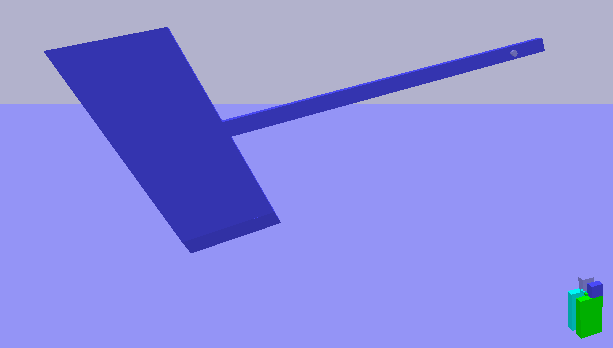
\includegraphics[height=2.3cm]{figs/article-charpy-1}
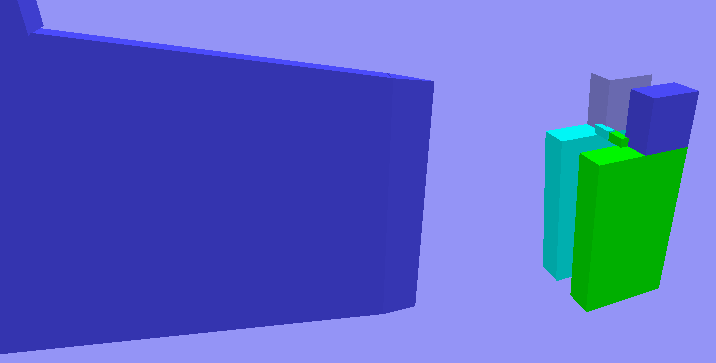
\includegraphics[height=2.3cm]{figs/article-charpy-2}
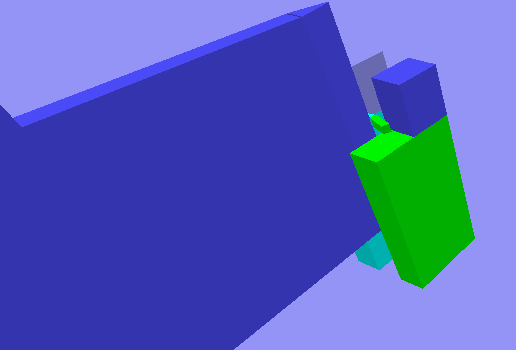
\includegraphics[width=8.65cm]{figs/article-charpy-3}
\caption{Detailed pictures from simulation of a Charpy impact test}
\label{fig:charpy-series}
\end{figure}

Table \ref{tab:ep2ts} shows energy loss for a few timesteps to demonstrate the sensitivity of the solution
using  elastic-plastic constraint 2.

\begin {table}
\tbl {Energy loss for few timesteps}{
\begin{tabular}{| c| c|l|}
\hline
{\bf Timestep[ms]} & {\bf Energy loss [J]} & {\bf Notes} \\ \hline
 0.2 &  170 & specimen penetrates hammer  \\ \hline
 0.1 &  120 & \\ \hline
 0.05 &  150 & \\ \hline
\end {tabular}}
\label{tab:ep2ts} 
\end {table}

Figure \ref{fig:charpy} shows an overview from simulation as the specimen passes between the supports.

\begin{figure}
\centering
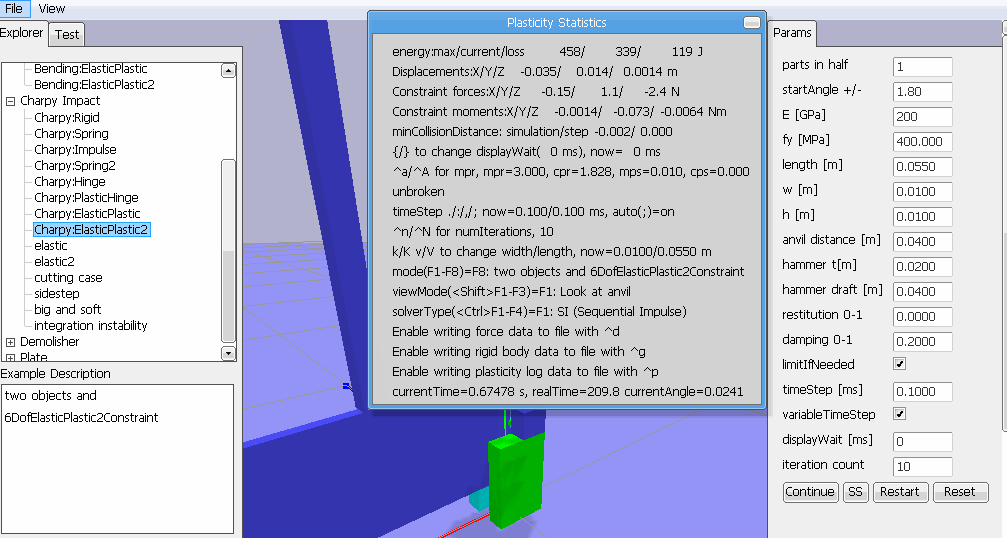
\includegraphics[height=4.5cm]{figs/article-charpy}
\caption{Overview of simulation of Charpy impact test}
\label{fig:charpy}
\end{figure}


\subsection{Demolisher}
The third numerical example introduces the demolisher.
The demolisher is a collection of possible scenarios that can be added to games to provide ductile joints between
rigid bodies.  Rigid concrete bodies are connected by steel enforcement.
Concrete density is 2000 $\frac{kg}{m^3}$ and steel density is 7800 $\frac{kg}{m^3}$. 
Steel is assumed to handle load. Yield stress of steel is 200 MPa.
Gravity is 10  $\frac{m}{s^2}$. Simulation step is $\frac{1}{60} $ s and 10 
iterations are done for a single step. Multiple simulation steps are done for each render if needed.

The simulation can be done in real time on modest hardware, e.g. 
on laptop having 2.0 GHz Intel i3 CPU with integrated graphics. 
Figure \ref{fig:demolisher} shows three screenshots from the simulation.

\begin{figure}
\centering
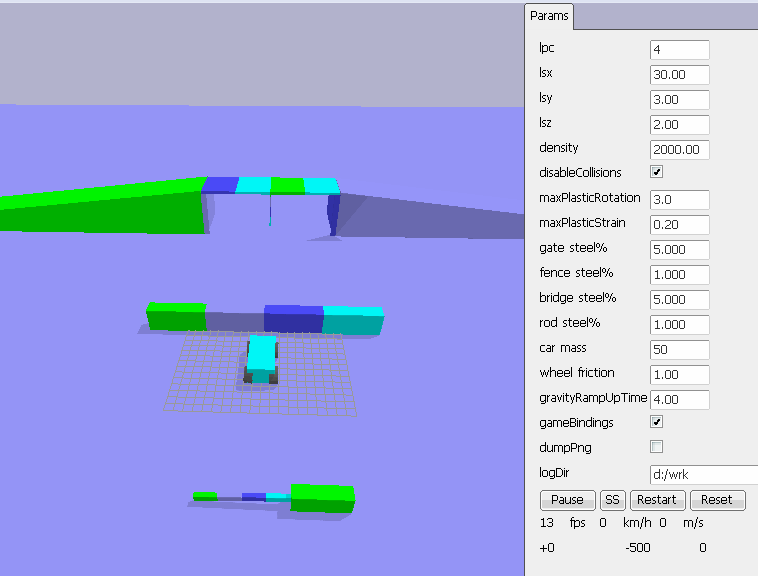
\includegraphics[width=8.65cm]{figs/demolisher-pre}
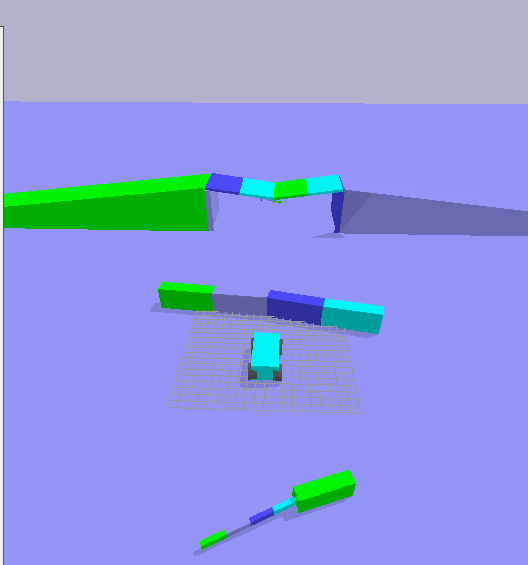
\includegraphics[height=4.3cm]{figs/demolisher-wip}
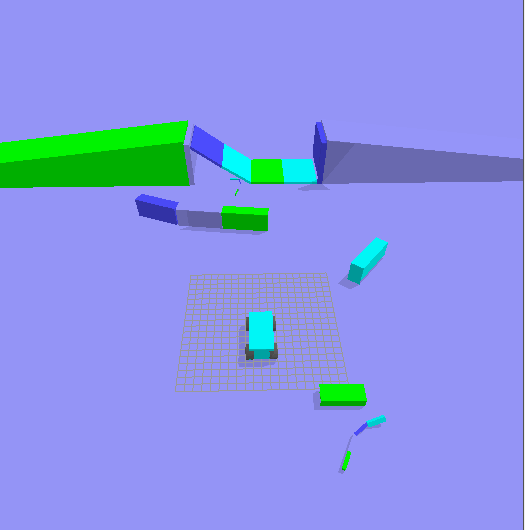
\includegraphics[height=4.3cm]{figs/demolisher-done}
\caption{Simulation of Demolisher scenario}
\label{fig:demolisher}
\end{figure}

The vehicle is modelled as a single box btRaycastVehicle with four driving wheels. Wheels are rendered for visual feedback.
In the left picture, the initial state is shown. 
The gate in front is modelled to be so slender that it has visible elastic deflection.
The gate support is modelled as a heavy box.
The bridge has rigid ramps and supports at both ends.
Gravity is applied gradually to avoid collapse of bridge at the start of the simulation.
In the middle picture, the bridge is shown in a state where a car has driven once over the bridge without stopping and
other bodies have taken light damage.
In the right picture, two joints have been broken and the bridge has fallen from teh support due to bending.


%\section{Simulation of Charpy impact test using \bullet}
\label{sec:bullet-charpy}

In following sections various methods for handling plasticity are described.
As physics engines have not been traditional area of research for plasticity, 
well known Charpy impact test was selected to be used as primary scenario
although it is against first two tips in \bullet Manual.

\begin{itemize}
\item Avoid very small and very larger collision shapes
\item Avoid large mass ratios
\end{itemize}

\subsection{Introduction to constraint processing in \bullet}
Constraint processing in \bullet is based on ODE, \cite{ode}.
Mathematical background and detailed examples are available by \cite{ode.joints}.
Equations \ref{eq:constraintEquation}, \ref{eq:lambdaLow} and
\ref{eq:lambdaHigh} 
are created for each constraint.

\begin{equation} \label{eq:constraintEquation}
J_1 v_1 + \Omega_1 \omega_1 + J_2 v_2 + \Omega_2 \omega_2 = c + C \lambda
\end{equation}

\begin{equation} \label{eq:lambdaLow}
\lambda \geq l
\end{equation}

\begin{equation} \label{eq:lambdaHigh}
\lambda \leq h
\end{equation}

Main parameters  and corresponding fields in \bullet 
 are described in table \ref{tab:constraintParameters}.

\begin {table}[htb!]
\begin{center}
\begin{tabular}{|c| l| l|}
\hline
{\bf Parameter} & {\bf Description} & {\bf btConstraintInfo2 pointer}\\  \hline
$J_1$ & Jacobian & m\_J1linearAxis, m\_J1angularAxis \\ 
$J_2$ & & m\_J2linearAxis, m\_J2angularAxis \\ \hline
$v$ & linear velocity & \\ \hline
$\omega$ & angular velocity & \\ \hline
$c$        &  right side vector   & m\_constraintError \\ \hline
$C$  & constraint force mixing & cfm \\  \hline
$\lambda$ & constraint force &  \\ \hline
$l$ & low limit for constraint force & m\_lowerLimit \\ \hline
$h$ & high limit for constraint force & m\_upperLimit \\ \hline
\end {tabular}
\end{center}
\caption {Constraint parameters} \label{tab:constraintParameters} 
\end {table}

\subsection{Common data}

\subsubsection{Material}

Material is steel. Density is 7800 $kg\over{m^{3}}$. Young’s modulus is 200 GPa. Yield stress is initially 400 MPa but it can be modified.

\subsubsection{Coordinate system}

X axis is horizontal, positive to direction where hammer comes from (left)\\
Y axis is vertical, positive up\\
Z axis is horizontal and Z=0 is symmetry plane

\subsubsection{Specimen}
Specimen dimensions can modified. Basic measures are 10x10x55 mm with 2 mm notch in middle which is taken into account in calculations. Specimen is positioned symmetrically around z=0, bottom at y=0.2 m and backside at x=0. 
Expected energy loss is product of plastic moment of section, hinge angle needed for specimen to go through supports and 
ultimate tensile strength of specimen. For hinge angle of 1.9 radians and ultimate tensile strength of 400 MPa expected energy 
loss is 122 J. Mass is about 40 g and in most cases it is modelled as two 20 g items. In laboratory tests variation for similar 
specimens is roughly about 10 %; see e.g. http://www.npl.co.uk/upload/pdf/cop06.pdf
Specimen can be subdivided to multiple parts.

\subsubsection{Support anvils}
Support anvils initially have 40 mm open space between them. Their width is 40 mm. 
If specimen bends about 1.9 radians (108 degrees) it will go between anvils. Space between anvils can be changed.

\subsubsection{Hammer}
Hammer is 0.5 m wide and 0.25 m high, thickness is 0.02 m. Mass is 19.5 kg. Hammer and hinge are positioned so that 
impact is horizontal  (global x-direction). Hammer arm is 40x40x500 mm. Hammer thickness can be changed.
Setting it to zero causes hammer not to get added to model. Hammer has modifiable draft. Default value is 0.04 m. 
Arm and draft are not taken into account for mass and inertia calculation.

\subsubsection{Energy calculation}

Energy for whole system is calculated so that potential energy and kinetic energy are calculated in updateEnergy. 
When hammer is resting in low position, energy is 64 J. 

\subsubsection{Breaking of constraints between objects}
For standard \bullet constraints breakingImpulseThreshold (BITh) can be defined. If impulse is larger than set limit constraint is activated. 
This allows object breaking to be simulated with very cheap calculation. 
This method is too simplified for ductile material and developing more precise methods in main objective of this work.  

\subsubsection{Timestep}

Usually bullet simulations are done using fixed time step of 1/60 s i.e. 16.67 ms. 
For this case 17 ms is too large timestep even to keep system stable. For impact time much smaller timestep is needed. 
Real time simulation was tried as option but was removed from code as it did not provide good results.  
Default time step was selected to be 5 ms outside impact time and 0.1 ms during impact. 
Automatic time stepping routine changes timestep so that at angles higher than 0.2 5 ms time step is
used and adjusts it linearly to selected time step between angles of 0.2 and 0.05. If specimen is no
longer at anvil larger timestep is also used.

\subsection{Single rigid body}
This is basic reference case without plasticity. Specimen should stop hammer.

\subsection{Constraint with zero limits}
In this case btGeneric6DofConstraint is used with high and low limits set to zero. 
Constraint is made breakable by setting breakingImpulseThreshold.
This is common technique to provide breakable objects in games and provides visually accetable results for brittle materials.

\subsection{SpringConstraint}
This shows how btGeneric6DofSpringConstraints act in case like this. 
Specimen can absorb very little elastic energy so rotational spring constants are calculated using plastic state i.e.
$W=bh^2/4$ where h=b-0.002m and yield stress is used instead of Young’s modulus for rotational springs.

\subsection{Spring2Constraint}
This basically same as SpringConstraint but uses newer btGeneric6DofSpring2Constraint which has recently appeared in
\bullet. 
Automatic stiffness limitation helps to avoid instability but may make constraint too soft.

\subsection{Hinge constraint with motors}
In this case btHingeConstraint is used.
Angular motor is enabled with target velocity of 0 and maximum motor impulse is set to
be plastic moment multiplied by timestep so that motor resists any rotation.

\subsection{PlasticHingeConstraint}
In this case new btPlasticHingeConstraint is used.
It is modification of btHingeConstraint and was is developed during this work.
PlasticHingeConstraint has additional fields for plasticMoment and previousHingeAngle and 
getAbsorbedEnergy method which returns product of plasticMoment and hingeAngle change.

\subsubsection{MaxPlasticRotation}
MaxPlasticRotation is new term which was introduced to allow efficient way to express ultimate strain in bending.
Implemented constraint has additional fields for maxPlasticRotation and currentPlasticRotation. 
After each step in which rotation angle changes, absolute value of 
angle change is accumulated to currentPlasticRotation. As currentPlasticRotation 
reaches maxPlasticRotation constraint is inactivated and specimen breaks. 
For ductile behaviour maxPlasticRotation could be set to e.g. 3-6 (radians) and for brittle
 behaviour to e.g.0.01-0.1 radians. MaxPlasticRotation is basically rotational stretch under bending moment.
 Basic sample can be tried using paperclip. It can typically handle two bend overs before breaking. 
Sewing machine needle or tooth pick which has same diameter is much harder to bend and it 
often breaks before plastic deformation takes place. 

\subsubsection{Limiting maximum moment in constraint}
btPlasticHingeConstraint::getInfo2InternalUsingFrameOffset is modified so that in case of lostop=histop, 
plasticMoment*timeStep is used as upper and lower limit instead of SIMD\_INFINITY. 

\subsection{ElasticPlasticConstraint}
In this case new bt6DofElasticPlasticConstraint is used.
It is based on SpringConstraint with some modifications

\begin{itemize}
\item internalUpdateSprings is modified so that nonlinear relation between displacements and forces can be defined. 
 If force is smaller than maximum force or moment for given degree of freedom,
  elastic behavior is handled in similar way as spring works. 
  If force is larger, maximum force is used. 
\item constraint breaks if active forces are high enough and plastic reserve has been used
\item frequency ratio of lowest mode and integration is used to limit spring functionality to avoid stability issues. 
 Ratio defines how many steps are needed for one period. 
 If number of integration steps is too low, spring is modified to ignore elastic part.
\end{itemize}

\subsection{ElasticPlastic2Constraint}
This is basically same as elasticPlasticConstraint but uses new bt6DofElasticPlastic2Constraint 
which is based on btGeneric6DofSpring2Constraint.
Get\_limit\_motor\_info2, setAngularLimits and setLinearLimits which are called by getInfo2 are modified. 
SIMD\_INFINITY values are replaced by maximum force values which are transformed to
corresponding impulsed by multiplying forces by integration interval.
btGeneric6DofSpring2Constraint has option limitIfNeeded for stiffness and damping to avoid issues. 
Spring is softened so that 4 steps are used for one step. This is not realistic for typical steel structures. 
In bt6DofElasticPlastic2Constraint plasticity code is activated if frequency is too high for stable solution.
If plasticity is activated due to large spring force or due to high frequency forces constraint error is 
calculated in similar way as for case where upper limit equals lower limit, (m\_currentLimit==3).

\section{Charpy impact test results using \bullet}
\label{sec:bullet-charpy-results}

\subsection{Results for single rigid body}
Timestep of 0.1 ms provides expeced results and specimen bounces hammer back.
Larger timesteps produce various kinds of unexpected results like
\begin{itemize}
\item Specimen goes trough anvil and penetrates hammer
\item Specimen moves sideways and stays on anvil. This can be seen e.g. by setting timestep to 17 ms and leaving hammer draft away.
\end{itemize}

\subsection{Results for constraint with zero limits}
This technique provides effective and stable way to simulate breaking into two objects. 
Required energy to break constraint can be controlled using
breakingImpulseThreshold. 

\subsection{Results for springConstraint}
Energy loss is in right scale but visual feedback is not realistic as specimen gets back to initial shape.
Unstable simulation can be seen by setting yield stress to e.g. 800 MPa.

\subsection{Results for spring2Constraint}
Results are quite similar as for springConstraint but automatic parameter tuning helps in avoiding unstable simulations.



\cleardoublepage

%\section{Discussion}

\subsection{Future work}
\label{subsec:futureWork}

\subsubsection{Implementation using GPU}
\bullet\ can already utilize GPU for many operations. 
Analysis on possible issues in used interfaces should be done before integrations.

\subsubsection{Acceptance to current physics engines}

Required work depends on selected dynamics engine. Availability of these features makes similar 
implementation possible.

\begin{itemize}
\item generic spring or motor constraint is already available 
\item possibility to update constraints after each simulation step
\end{itemize}

Current implementation is done based on \bullet\ but it still needs refactoring and testing before it can be 
accepted to main stream. Interfaces should be reafctored so that handling of additional features like large 
displacements and material nonlinearity can be implemented without further changes.

\subsubsection{Large displacements}
Large displacements are typical if plasticity is involved and
large displacements can also take place due to rigid body motion and should be taken into account.

Update of constraints can be done in  many ways but using callbacks allows clean integration i.e. no changes
to solver core are needed.
In \bullet\ there are already three per step callbacks. 

\begin{itemize}
\item updateActions
\item updateActivationState
\item btInternalTickCallback
\end{itemize}

\demolisher already uses updateActions and that seems 
good way to do also other updates. Special care should be taken to avoid unnecessary updates.

\subsubsection{Material nonlinearity}
Update of constraint properties can be done in callbacks in similar way as for large displacements.
Material definition should be defined so that stress-strain curve can be defined as array of pairs.
This is probably not significant feature for simulations in gaming area but interesting feature for research and teaching area.

\subsection{Object subdivision just in time}
Just in time activation could avoid extra overhead from multiple objects and constraints.
Impacts causing plasticity are usually quite brief and they happen at distinct times. 
Simulation could allocate processing units for handling these and release them after impact has been processed.

\cleardoublepage


\fancyhead[LO]{\nouppercase{\bfseries\firstleftxmark}}%
\fancyhead[RE]{\nouppercase{\bfseries\lastrightxmark}}%
\extramarks{}{References}   % this will remove the "References" to be appearing at the header at first page of bibliography
\extramarks{References}{References}
\bibliography{ref}%
\bibliographystyle{LUTapa}%

%\cleardoublepage %

\end{document}
